% Author: Jannes Bantje
% Modified: Lars Haalck lars.haalck@wwu.de
% please ask Lars Haalck first if you have any questions
%!TEX root = thesis.tex
% Author: Jannes Bantje
% Modified: Lars Haalck lars.haalck@wwu.de
% please ask Lars Haalck first if you have any questions

\documentclass[%
a4paper,
parskip=half,
index=totoc,
toc=listof,
fontsize=11,
headinclude,
twoside,
BCOR=12mm,
cleardoublepage=empty,
DIV=13,
draft=false % delete this line completely to remove all todos
]{scrreprt}



\usepackage[usenames,x11names]{xcolor}
\usepackage[final]{graphicx}
\usepackage{subcaption}

% typographic settings, fonts, and math
\usepackage[utf8]{inputenc}
\usepackage[lining,semibold]{libertine}
\usepackage[T1]{fontenc}
\usepackage{textcomp} % verhindert ein paar Fehler bei den Fonts
\usepackage[varl]{zi4}
\usepackage{mathtools,amssymb,amsthm} % Verbesserung von amsmath (die amsmath selbst lädt)
\usepackage[libertine,cmintegrals,bigdelims,varbb]{newtxmath}
\usepackage[ngerman]{babel}
\usepackage[babel=true, tracking=true,final]{microtype}
\usepackage[ngerman]{datetime}



% set line spacing
\usepackage{setspace}
% for example 1.5 line spacing
\onehalfspacing

% literature settings
\usepackage[%
backend=biber,
sortlocale=auto,
natbib,
hyperref,
backref,
mincitenames=1,
maxcitenames=1,
style=ieee
]%
{biblatex}
\addbibresource{literature.bib} % sets literature file

% hyperref settings to make links clickable in PDF
\usepackage[%
hidelinks,
pdfpagelabels,
bookmarksopen=true,
bookmarksnumbered=true,
linkcolor=black,
urlcolor=SkyBlue2,
plainpages=false,
pagebackref,
citecolor=black,
hypertexnames=true,
pdfborderstyle={/S/U},
linkbordercolor=SkyBlue2,
colorlinks=false,
backref=false
]{hyperref}
\hypersetup{final}

% enumeration settings
\usepackage[shortlabels]{enumitem}
\setlist[enumerate,description]{font=\sffamily\bfseries} % makes labels in enumeration bold
\usepackage[german=quotes]{csquotes}

% allows adding of todo notes at the side of the document
\setlength{\marginparwidth}{0.8cm}
\usepackage[obeyDraft,textsize=tiny,textwidth=1.2cm]{todonotes}

% settings for the header and footer
\usepackage[headsepline=1pt]{scrlayer-scrpage}
\pagestyle{scrheadings}
\clearscrheadfoot % clear defaults
\setkomafont{headsepline}{\color{gray}} % adds a gray line under the header

% set section title on the right, and chapter title on the left page in a double page
% document
\automark[section]{chapter}

\rohead{\rightmark} % section title on the right side
\lehead{\scshape\leftmark} % chapter title on the left side an in small caps
\ofoot[\pagemark]{\pagemark} % page marks always on the outer site of the page

% sets page marks and footer and header texts to sans-serif in gray
\renewcommand*{\pnumfont}{\sffamily}
\renewcommand*{\footfont}{\sffamily\color{gray}}
\renewcommand*{\headfont}{\sffamily\color{gray}}

% change the chapter, section and subsection font sizes and spacings a bit for a5 format
% \setlength{\footskip}{1.75\baselineskip} % change the spacing a bit for a5 format
% \RedeclareSectionCommand[%
% afterskip=1\baselineskip,%
% beforeskip=-1\baselineskip]{chapter}

% \setkomafont{chapter}{\LARGE}
% \setkomafont{section}{\Large}
% \setkomafont{subsection}{\large}

% adds a thick gray line after the chapter number
\renewcommand*{\chapterformat}{%
    \thechapter\enskip
    \textcolor{gray!50}{\rule[-\dp\strutbox]{1.5pt}{\baselineskip}}\enskip
}


% math environments
\usepackage{amsthm}
\usepackage{thmtools}
\usepackage{mdframed}
\usepackage{blindtext}
\renewcommand{\listtheoremname}{Übersicht aller Aussagen}

% -- Theoreme als PDF-Lesezeichen
\usepackage{bookmark}
\bookmarksetup{open,numbered}
\makeatletter
\newcommand*{\theorembookmark}{%
    \bookmark[
    dest=\@currentHref,
    rellevel=1,
    keeplevel,
    ]{%
        \thmt@thmname\space\csname the\thmt@envname\endcsname
        \ifx\thmt@shortoptarg\@empty
            \else
                \space(\thmt@shortoptarg)%
            \fi
        }%
    }
\makeatother

% -- Definition der einzelnen Umgebungen
\declaretheoremstyle[%
headfont=\sffamily\bfseries,
notefont=\normalfont\sffamily,
bodyfont=\normalfont,
headformat=\NAME\ \NUMBER\NOTE,
headpunct=,
postheadspace=\newline,
spaceabove=\parsep,spacebelow=\parsep,
%shaded={bgcolor=gray!20},
postheadhook=\theorembookmark,
mdframed={
    backgroundcolor=gray!20,
    linecolor=gray!20,
    innertopmargin=6pt,
    roundcorner=5pt,
    innerbottommargin=6pt,
    skipbelow=\parsep,
skipbelow=\parsep }
]%
{mainstyle}

\declaretheoremstyle[%
headfont=\sffamily\bfseries,
notefont=\normalfont\sffamily,
bodyfont=\normalfont,
headformat=\NAME\ \NUMBER\NOTE,
headpunct=,
postheadspace=\newline,
spaceabove=15pt,spacebelow=10pt,
postheadhook=\theorembookmark]%
{mainstyle_unshaded}

\declaretheoremstyle[%
headfont=\sffamily\bfseries,
notefont=\normalfont\sffamily,
bodyfont=\normalfont,
headformat=\NUMBER\NAME\NOTE,
headpunct=,
postheadspace=\newline,
spaceabove=15pt,spacebelow=10pt,
% shaded={bgcolor=gray!20},
postheadhook=\theorembookmark]%
{mainstyle_unnumbered}

\declaretheorem[name=Definition,parent=section,style=mainstyle]{definition}
\declaretheorem[name=Definition,numbered=no,style=mainstyle]{definition*}
\declaretheorem[name=Definition,sharenumber=definition,style=mainstyle_unshaded]{definitionUnshaded}

\declaretheorem[name=Theorem,sharenumber=definition,style=mainstyle]{theorem}
\declaretheorem[name=Theorem,numbered=no,style=mainstyle_unnumbered]{theorem*}

\declaretheorem[name=Proposition,sharenumber=definition,style=mainstyle]{proposition}
\declaretheorem[name=Lemma,sharenumber=definition,style=mainstyle]{lemma}

\declaretheorem[name=Satz,sharenumber=definition,style=mainstyle]{satz}
\declaretheorem[name=Satz,sharenumber=definition,style=mainstyle_unshaded]{satzUnshaded}
\declaretheorem[name=Satz,numbered=no,style=mainstyle_unnumbered]{satz*}

\declaretheorem[name=Korollar,sharenumber=definition,style=mainstyle]{korollar}

\declaretheorem[name=Notation,numbered=no,style=mainstyle_unnumbered]{notation}
\declaretheorem[name=Bemerkung,numbered=no,style=mainstyle_unnumbered]{bemerkung}
\declaretheorem[name=Beispiel,numbered=no,style=mainstyle_unnumbered]{beispiel}
\declaretheorem[name=Beispiele,numbered=no,style=mainstyle_unnumbered]{beispiele}


%Informationen zur Arbeit
\newcommand{\printname}{Sufian Zaabalawi, Hasan Can, Daniel König}
\newcommand{\printgroup}{Gruppe 1}
%\newcommand{\printnumber}{XXX XXX}

\newcommand{\printtitle}{Predicting COVID-19 in X-ray Images}
\newcommand{\printcity}{Münster}
\newcommand{\printtype}{Praktikum}
\newcommand{\printdegree}{Mustererkennung}
%\newcommand{\printsupervisor}{John Doe}
%\newcommand{\printfirstassessor}{Prof. Dr. Erika Musterfrau}
%\newcommand{\printsecondassessor}{Prof. Dr. Hans Peter}
\newcommand{\printinstitute}{Fachbereich Mathematik und Informatik \\
Institut für Informatik}

\usepackage{graphicx}
% !!!only for pseudo text, can be deleted!!!
\usepackage{blindtext}

\begin{document}
% set the pager numbering to big roman numbers for firt few pages
\pagenumbering{Roman}
\listoftodos

% titlepage does not need cleardoubleoddemptypage
\begin{titlepage}
	\thispagestyle{empty}

\begin{center}
    
\includegraphics[width=7.5cm]{logos/wwu-logo.eps}
    \par
    \vspace*{8ex}
    \LARGE
    \printtitle
    \par
    \normalsize
    \vspace*{8ex}
    \large
    \textsc{\printtype}\\
    \normalsize
    zur Vorlesung\\
    \large
    \textsc{\printdegree}
    \par
    \normalsize
    \vspace*{6ex}
    Westfälische Wilhelms-Universität Münster\\
    \printinstitute
\end{center}

%\par
%\vspace*{6ex}
%Betreuung:\\
%\large
%\textit{\printsupervisor}
%
%\par
%\normalsize
%\vspace*{2ex}
%Erstgutachter:\\
%\large
%\textit{\printfirstassessor}
%
%\par
%\normalsize
%\vspace*{2ex}
%Zweitgutachter:\\
%\large
%\textit{\printsecondassessor}

\vspace*{5cm}
\par
\normalsize
\vspace*{2ex}
Eingereicht von:\\
\large
\textit{\printname}\\
\textit{\printgroup}

\par
\normalsize
\vspace*{4ex}
\printcity, \makeatletter
\monthname
\makeatother~\the\year

\end{titlepage}

\tableofcontents

% set the page numbering back to arabic
\pagenumbering{arabic}
\setcounter{page}{1}
%!TEX root = ../documentation.tex
\chapter{Einleitung}
\label{ch:einleitung}

In Dezember 2019 ist ein Virus in Wuhan, China, ausgebrochen welcher dann Coronavirus (SARS-CoV-2), bzw. Covid-19 genannt wurde. Dieser Virus ist eine Lungenkrankheit, welche oft eine Pneunomie auslöst. Er hat sich erst aus dem Gebiet (Wuhan) in das ganze Land China ausgebreitet und fing dann nach 2-3 Monaten an, sich auch in andere Länder zu verbreiten. Dieser Anstieg war so rapide, dass bis mitte April schon mehr als 2 Millionen Menschen infiziert wurden und 150.000 von diesen gestorben sind. Inzwischen zum Zeitpunkt Oktober, sind diese Zahlen sogar auf 35 Millionen Infektionen und davon 1 Millionen Todesfälle. An diesen Zahlen erkennt man sehr schnell, dass dieses Virus sehr ernst zu nehmen ist. Um diese Zahlen möglichst gering zu halten, ist das schnelle und richtige diagnostizieren der Krankheit wichtig. Hierfür gibt es verschiedene Methoden, wobei die am häufigsten angewandte Methode über eine Probe des Rachens verläuft. Mit dieser Methode dauert es in der Regel etwa 48 Stunden, bis man die Ergebnisse hat, weswegen man weiter forscht, um vorallem auch eine höchstmögliche Genauigkeit beizubehalten, zusätzlich zu einem schnellen Ergebnis. Da diese Erkrankung eine Lungenkrankheit ist, hat man sich in Studien Röntgenbilder der Lunge angeguckt und Covid-19 Patienten mit Patienten ohne Covid-19 verglichen. Hierbei ist aufgefallen, dass der Virus Abnormalitäten auf der Lunge hinterlässt, welche dann im Röntgenbild zu erkennen sind. Dies führt dann zu der Idee, ein Deep Learning Modell aufzustellen, welches trainiert wird, so dass möglichst viele Patienten schnell und genau diagnostiziert werden können.
\newline
Das ganze Projekt fängt dann damit an, dass man Bilder zum Trainieren und auch Testen des Modells benötigt. Jedoch, dadurch, dass der Virus noch relativ neu ist, gibt es leider nicht viele (öffentliche) Röntgenbilder, welche man benutzen könnte. Hier wurde von CheXpert\footnote{"CheXpert is a large dataset of chest X-rays and competition for automated chest x-ray interpretation, which features uncertainty labels and radiologist-labeled reference standard evaluation sets. https://stanfordmlgroup.github.io/competitions/chexpert/"}, welche ebenfalls ein Deep Learning Modell, mit einem passenden Paper dazu, aufgesetzt haben, ein Datenset von Bildern bereit gestellt. Dieses Datenset beinhaltet 2100 Röntgenbilder von Patienten, mitunter 100 an Covid-19 erkrankten Patienten.
\newline
Um mit diesem Datensatz weiter zu arbeiten, muss man diesen vorerst anpassen, da zum einen der Anteil der Covid-Bilder noch zu gering ist und zum anderen Störfaktoren bearbeitet werden müssen. Der Datensatz beinhaltet neben gesunden- und Covid Patienten auch anders erkrankte Patienten, zusätzlich zu Patienten mit Geräten im Körper, wie z.B. Herzschrittmacher. Da für uns in diesem Fall nur Covid-Patienten wichtig sind, müssen die anderen Faktoren durch passendes Augmentation (dazu mehr in späteren Kapiteln) und durch das Trainig raus gefiltert werden. Hierfür werden die Bilder bearbeitet, Noise entfernt, heller/dunkler gemacht und noch mehr in Kombination. Zusätzlich wurden alle Bilder auf eine Größe von 320x320 komprimiert, um Informationsverlust durch das vergrößern von einigen Bildern zu vermeiden. Im letzten Schritt muss der Datensatz vergrößert werden, hierfür benutzen wir Spiegelungen und leichte Zerrungen, um im Endhinein auf die gleiche Anzahl von Bildern zu kommen, mit 1: gesunden Patienten, 2: an Covid-19 erkrankten Patienten und 3: anders erkrankten Patienten.
\newline
Nach der Datenverabeitung werden die Modelle trainiert, hierbei haben wir uns verschiedene Modelle angeguckt und verglichen, so dass wir uns am Ende darauf entschieden haben das Modell ResNet und das Modell SqueezeNet zu benutzen (genaueres im Kapitel "Models"). Diese Beiden Modelle wurden dann so weit angepasst und ausgebessert, bis man diese vergleichen konnte, wobei in unserem Fall, SqueezeNet die höhere Genauigkeit geboten hat. Diese Ergebnisse stellen wir dann am Ende tabellarisch und grafisch dar, sowohl als Confusions-/Binär- Matrizen, als auch als Lernkurven, mit den passenden Ergebnissen.
\newline
Obwohl diese Ergebnisse bereits zufriedenstellend scheinen, kann man diese mit Sicherheit um einiges verbessern, indem man größere Datensätze zur Verfügung bekommt und mit diesen dann noch weiter experimentiert.
\newline
Der Rest dieser Ausarbeitung ist wie folgt gegliedert. Zunächst werden in Kapitel 3 die gegebenen Daten analysiert, um genau zu wissen was angepasst werden muss. So wird dann in Kapitel 4 die folgende Datenvorverarbeitung erklärt. In Kapitel 5 gibt es genauere Erklärungen zu den verwendeten und trainierten Modellen, um einen besseren Einblick zu bekommen, wie diese denn Funktionieren. Darauf folgt in Kapitel 6 das Eigentliche Training und in Kapitel 7 werden dann die ganzen Ergebnisse aufgezeigt, welche durch das ganze Projekt hindurch und vorallem am Ende gesammelt wurden. Abgeschlossen wird die Ausarbeitung mit einer Einleitung zum Ausführen der Skripte, gefolgt von der Literatur.



%!TEX root = ../documentation.tex
\chapter{Datenanalyse}
\label{ch:data_analysis}

\section{Bilddaten}
\newlength{\imagewidth}

Wir betrachten zunächst die Bilddaten aus dem Datenset und stellen anhand von geeigneten Beispielen und Analysen heterogene Eigenschaften dieser dar, welche sich für das Training als problematisch erweisen könnten.

\begin{figure}[ht]
	\centering
	\begin{subfigure}[b]{0.45\textwidth}
		\includegraphics[width=\textwidth]{../images/34308.jpeg}
		\caption{34308.jpeg\\Originalgröße 1524 x 1516 Pixel}
	\end{subfigure} \hfill
	\begin{subfigure}[b]{0.45\textwidth}
		\includegraphics[width=\textwidth]{../images/65415.jpg}
		\caption{65415.jpg\\Originalgröße 369 x 320 Pixel}
	\end{subfigure}
	\caption{Zwei Bilder männlicher Patienten aus dem Datenset}
\end{figure}

Die Beispiele (a) und (b) lassen einen deutlich unterschiedlichen Kontrast erkennen. Bei Beispiel (a) handelt es sich zudem um ein Farbbild während es sich bei Beispiel (b) um ein Schwarzweißbild handelt. Die beiden Bilder weisen unterschiedliche Dimensionen auf.\\
Diese heterogenen Eigenschaften zeigen Komplexität innerhalb des Datensets, welche von einem gelernten Model entsprechend wiedergespiegelt werden müsste. Es ist also angebracht die Daten mittels geeigneter Vorverarbeitung zu homogenisieren.

Insgesamt werden die Unterschiede in Dimension und Farbe von den folgenden Grafiken dargestellt.

\begin{figure}[H]
	\centering
	\settowidth{\imagewidth}{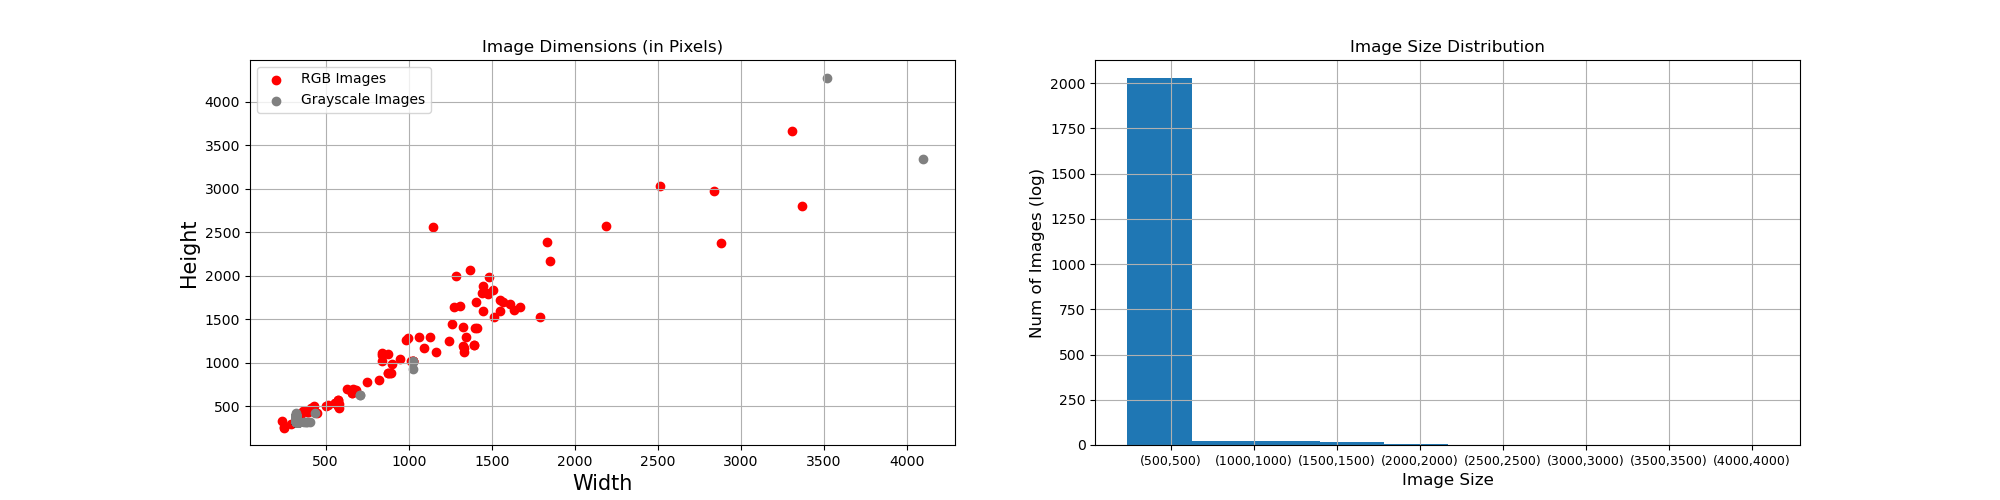
\includegraphics{../results/image_sizes.png}}
	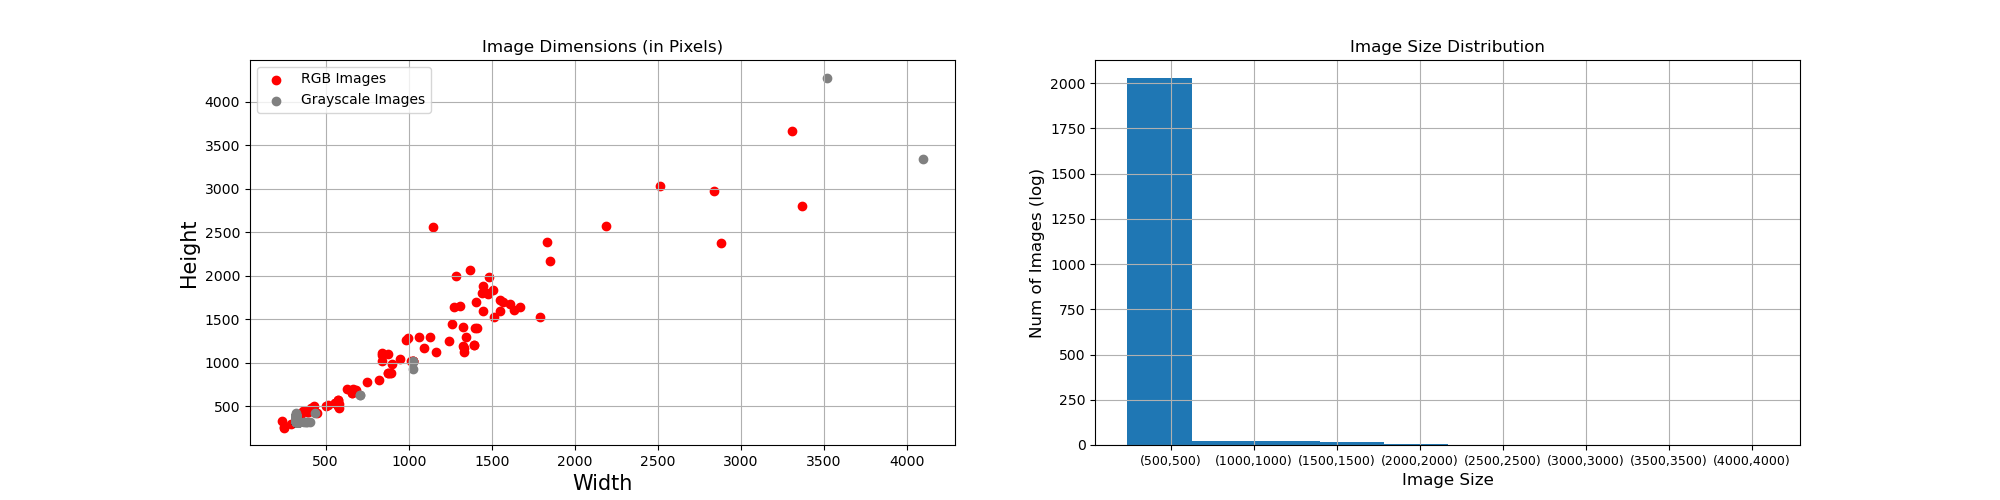
\includegraphics[trim=110px 0 0.5\imagewidth{} 0, clip,width=0.9\textwidth]{../results/image_sizes.png}
	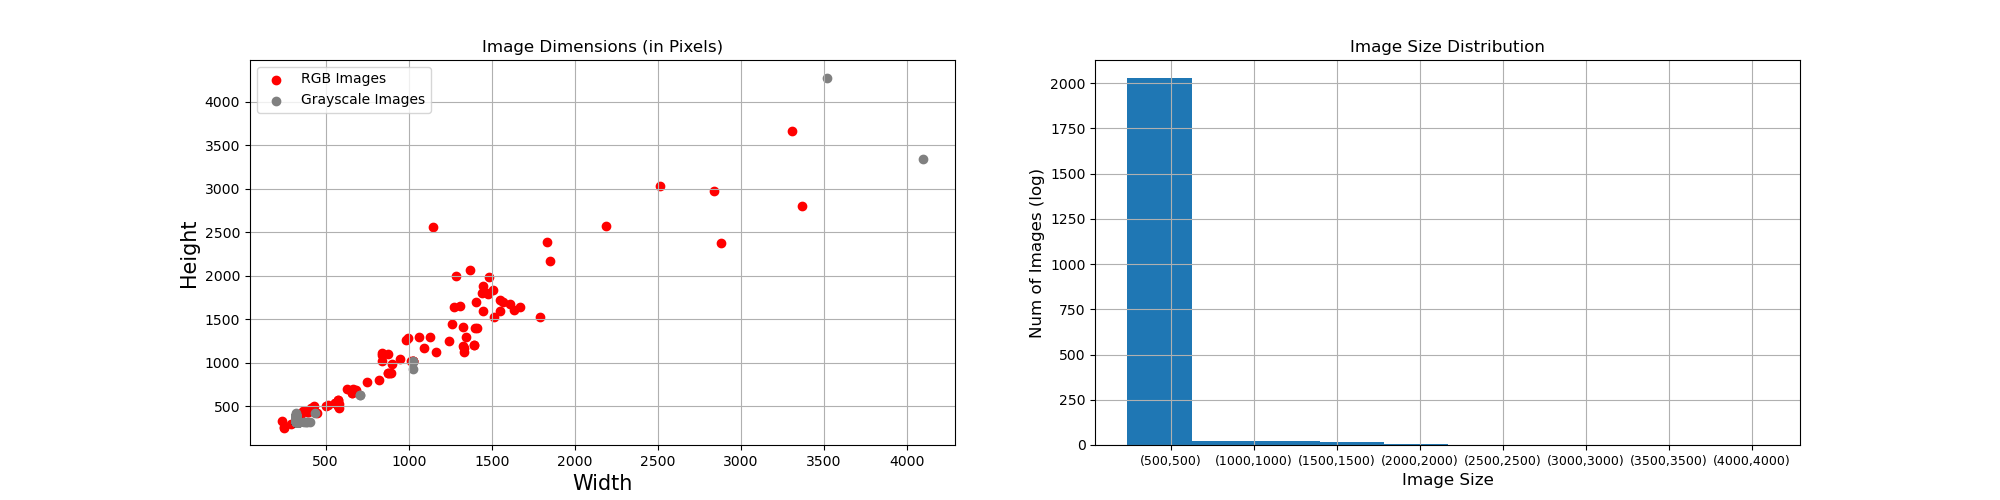
\includegraphics[trim=0.5\imagewidth{} 0 110px 0, clip,width=0.9\textwidth]{../results/image_sizes.png}
	\caption{Verteilung der Bilddimensionen}
\end{figure}

Von den Bildern sind 92 Farbbilder und 2008 Schwarzweißbilder. Ein Großteil der Dimensionen ist im Bereich von 320 x 320 Pixeln angeordnet.

\section{Klassen}

Wir betrachten nun die Verteilung der Klassen über das Datenset in zwei Konstellationen. In der ersten Konstellation wird jede Krankheit von einer eigenen Klasse repräsentiert, während in der zweiten Konstellation alle Krankheiten mit Ausnahme von COVID-19 zu einer Klasse zusammengefasst werden.

\begin{figure}[H]
	\centering
	\settowidth{\imagewidth}{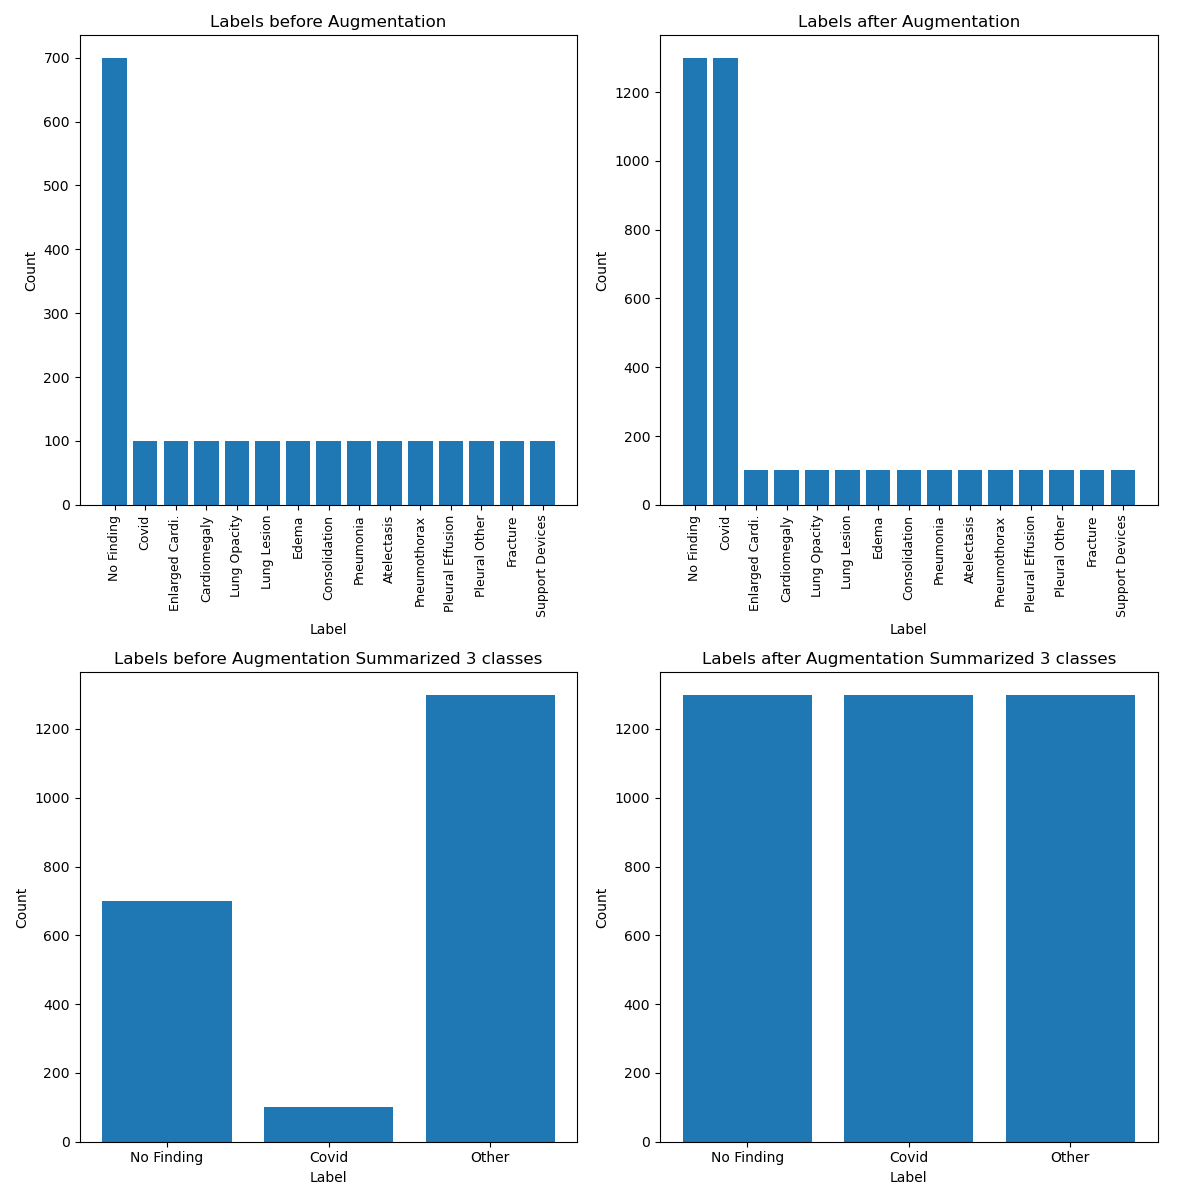
\includegraphics{../results/balancing.png}}
	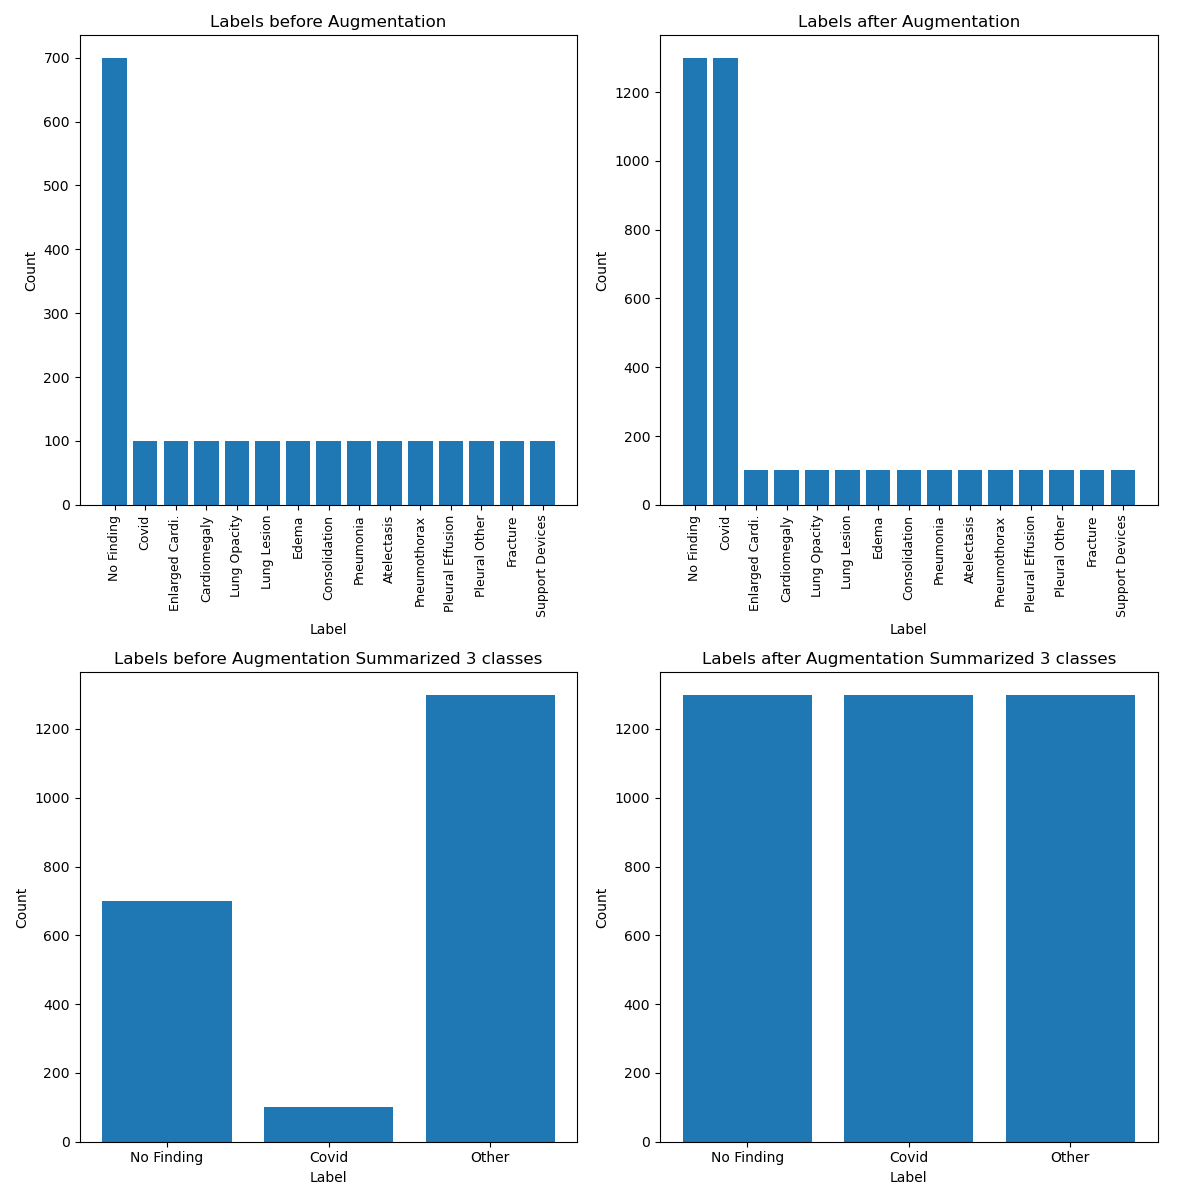
\includegraphics[trim=0 0 0.51\imagewidth{} 0, clip,width=0.3\imagewidth{}]{../results/balancing.png}
	\caption{Verteilung der Klassen}
\end{figure}

In der ersten Konstellation sind die Krankheiten gleichverteilt. Pro Krankheit existieren 100 Beispielbilder. Insgesamt existieren 1400 Bilder für die Krankheitsklassen und 700 ohne Befund.\\
In der zweiten Konstellation ist der Anteil an COVID-19 Erkrankungen im Vergleich zu den anderen Klassen relativ gering.
Um eine gute Generalisierungsfähigkeit sicherzustellen, ist es hier sinnvoll zusätzliche Trainingsbeispiele aus der COVID-19 Klasse bereitzustellen.

Wir betrachten ebenfalls die Verteilung der Features Alter und Geschlecht innerhalb der COVID-19 Erkrankungen aus dem Datenset.

\begin{figure}[ht]
	\centering
	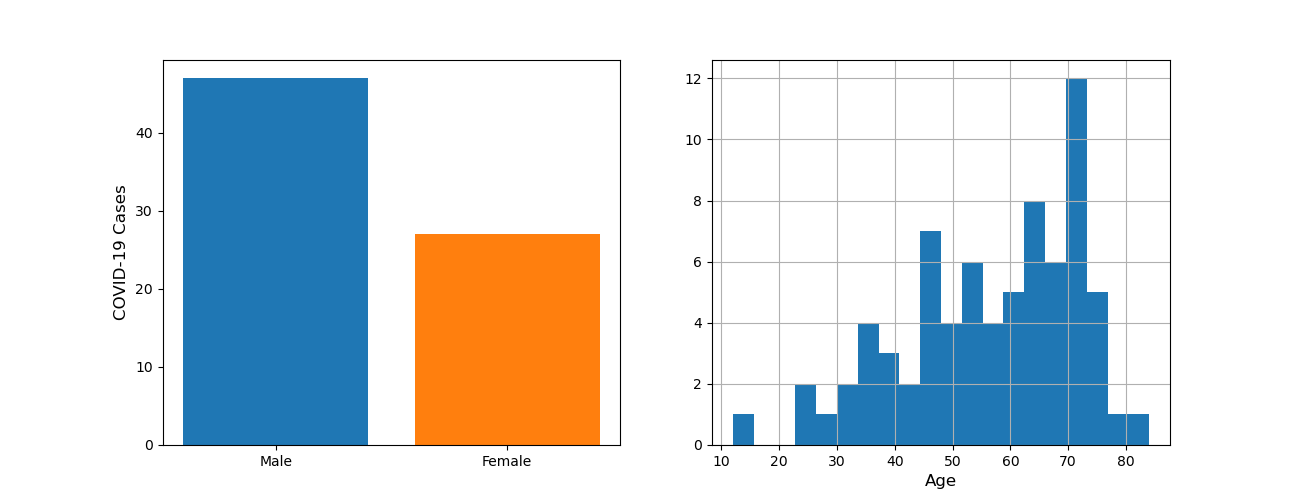
\includegraphics[width=\textwidth]{../results/features_analysis.png}
	\caption{Analyse der Features Alter und Geschlecht bei COVID-19 erkrankten Patienten}
\end{figure}

Die Anteile von männlichen Patienten ist höher als der von weiblichen. Ebenfalls sind Daten von eher älteren Patienten vorhanden. Das Durchschnittsalter beträgt 56,46 Jahre.\\
Eventuell sind zusätzliche Maßnahmen zur Entzerrung der Daten sinnvoll.
%!TEX root = ../documentation.tex
\chapter{Datenvorverarbeitung}
\label{ch:data_preprocessing}

\section{Bilddaten}

In der vorherigen Datenanalyse wurden folgende Probleme herausgestellt:

\begin{enumerate}
	\item{Dimensionsunterschiede}
	\item{Farbunterschiede}
	\item{Kontrastunterschiede}
\end{enumerate}

Diese sollen nun mit geeigneten Vorverarbeitungsschritten gelöst werden.

Die Bilder müssen als Eingabe für das Model in einer einheitlichen Größe vorliegen. Dazu skalieren wir alle Bilder auf den Mittelwert der Dimension von 384x384 Pixeln.\\
Da die farblichen Informationen in Röntgenbildern irrelevant sind, werden alle Bilder zu Schwarzweißbildern umgewandelt.\\
Weiterhin werden die Kontrastunterschiede über einen Histogrammausgleich verringert.

\begin{figure}[H]
	\centering
	\begin{subfigure}[b]{0.45\textwidth}
		\includegraphics[width=\textwidth]{../images/42081.jpg}
		\caption{Originalbild 42081.jpg\\1524 x 1516 Pixel}
	\end{subfigure} \hfill
	\begin{subfigure}[b]{0.45\textwidth}
		\includegraphics[width=\textwidth]{../train_data/42081.jpg}
		\caption{Vorverarbeitetes Bild\\384 x 384 Pixel}
	\end{subfigure}
	\caption{Vergleich eines Originalbildes mit dem daraus resultierenden vorverarbeiten Bild}
\end{figure}
\section{Models}
\label{ch:models}

Da es in der Regel nicht \textit{das} Perfekte Modell gibt um Klassen zu klassifizieren, haben wir hier verschiedene verglichen. Dabei haben wir uns hauptsächlich auf ResNet und SqueezeNet konzentriert, da diese beiden Modelle Erfahrungsgemäß, laut anderen Berichten, die höchste Accuracy hatten.
Damit man diese Netze jedoch nutzen kann, muss man erstmal wissen, wie genau sie funktionieren.

\subsection{ResNet152}

ResNet ist eine der beliebtesten CNN Architekturen, dadurch, dass es der Sieger der ImageNet competition in 2015 war. ResNet bietet einen einfachen \textit{gradient flow} für noch effizienteres Training.
\newline Die Hauptidee bei ResNet ist es einige Layers gezielt zu überspringen. Hierdurch kann das Netz einen direkten Weg zu den ersten layern aufbauen wodurch die gradient updates für diese Layer vereinfacht werden. Zudem gibt es verschiedene Versionen von ResNet, welche alle jedoch sehr ähnlich sind, sich nur in der Anzahl der Layer unterscheiden (ResNet18, ResNet50, ResNet152,..).
Dieses Modell wird in der folgenden Abbildung presäntiert(Als ResNet18 Version), muss dann jedoch mit anderen Modellen verglichen werden, um vorallem auch Faktoren wie Parameter etc. zu anzupassen.

\subsubsection*{}
\begin{figure}[h]
    \centering
    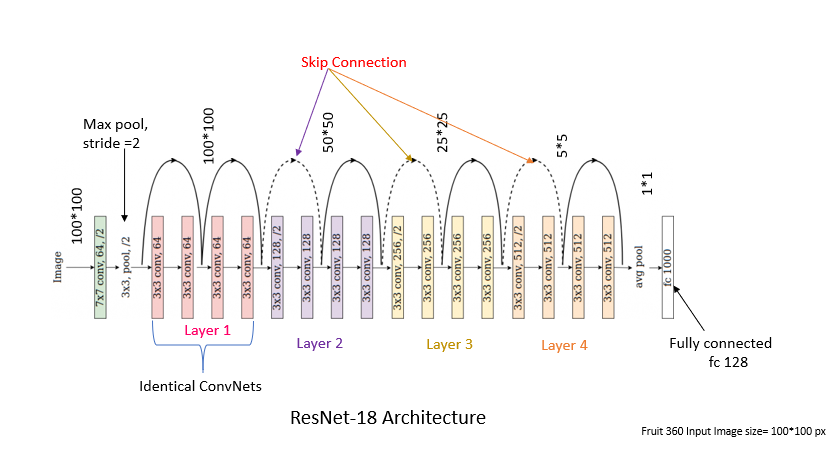
\includegraphics[width=1.1\textwidth]{Bilder/ResNet18Model.png}
    \caption{}
    \label{fig:ResNet18}
\end{figure}

\subsection{SqueezeNet}

SqueezeNet ist eine CNN Architektur und erreicht AlexNet-Genauigkeit auf ImageNet, mit 50x weniger Parametern. Mit zusätzlichen Funktionen zur Modell-Kompression, lässt sich SqueezeNet zudem auf weniger als 0.5MB verkleinern, somit 510x kleiner als AlexNet.
\newline Hierbei wird zu einem 1x1 Layer gewechselt, welches den Input in der vertikalen Dimension komprimiert, daher der Name \textit{squeeze}, gefolgt von insgesamt zwei paralellen 1x1 und 3x3 convolutional layern, wodurch die Tiefe der Daten wieder erweitert wird.
\newline Das Modell ist hierdurch klar, jedoch muss das komprimieren der Parameter genauer angeschaut werden, da es hierfür drei verschiedene Strategien gibt. Die erste hierbei ist 3x3 Filter durch 1x1 Filter auszutauschen, da ein 3x3 Filter 9x so viele Parameter hat wie ein 1x1 Filter. Als zweite Strategie wird die Anzahl der Eingabe-Kanäle, zu den 3x3 Filtern, reduziert. Da die Anzahl der Parameter wie folgt berechent wird: 
\newline (Anzahl der Eingabe-Kanäle) * (Anzahl der Filter) * (3*3)
Einen Faktor haben wir durch Strategie 1 bereits reduziert, bei Strategie 2 reduziert man somit einen weiteren Faktor, um somit das insgesamte Produkt der Parameter zu reduzieren. Hierbei werden oft \textit{squeeze layers} benutzt um die Anzahl der Eingabe-Kanäle zu reduzieren. Zuletzt die dritte Strategie, die verwendet wird, ist das späte \textit{downsample} im Netz, so dass die Convolution Layers große \textit{activation maps} haben. Da in einem Convolutional Netz jedes Convolution Layer ein \textit{output activation map} erzeugt, welche 1x1 oder größer ist und durch die größe der Eingabedaten der Wahl der layers bestimmt wird, werden diese durch \textit{downsample}, in der CNN Architektur, verkleinert. In der Folgenden Abbildung wird Architektur veranschaulicht.

\subsubsection*{}
\begin{figure}[h]
    \centering
    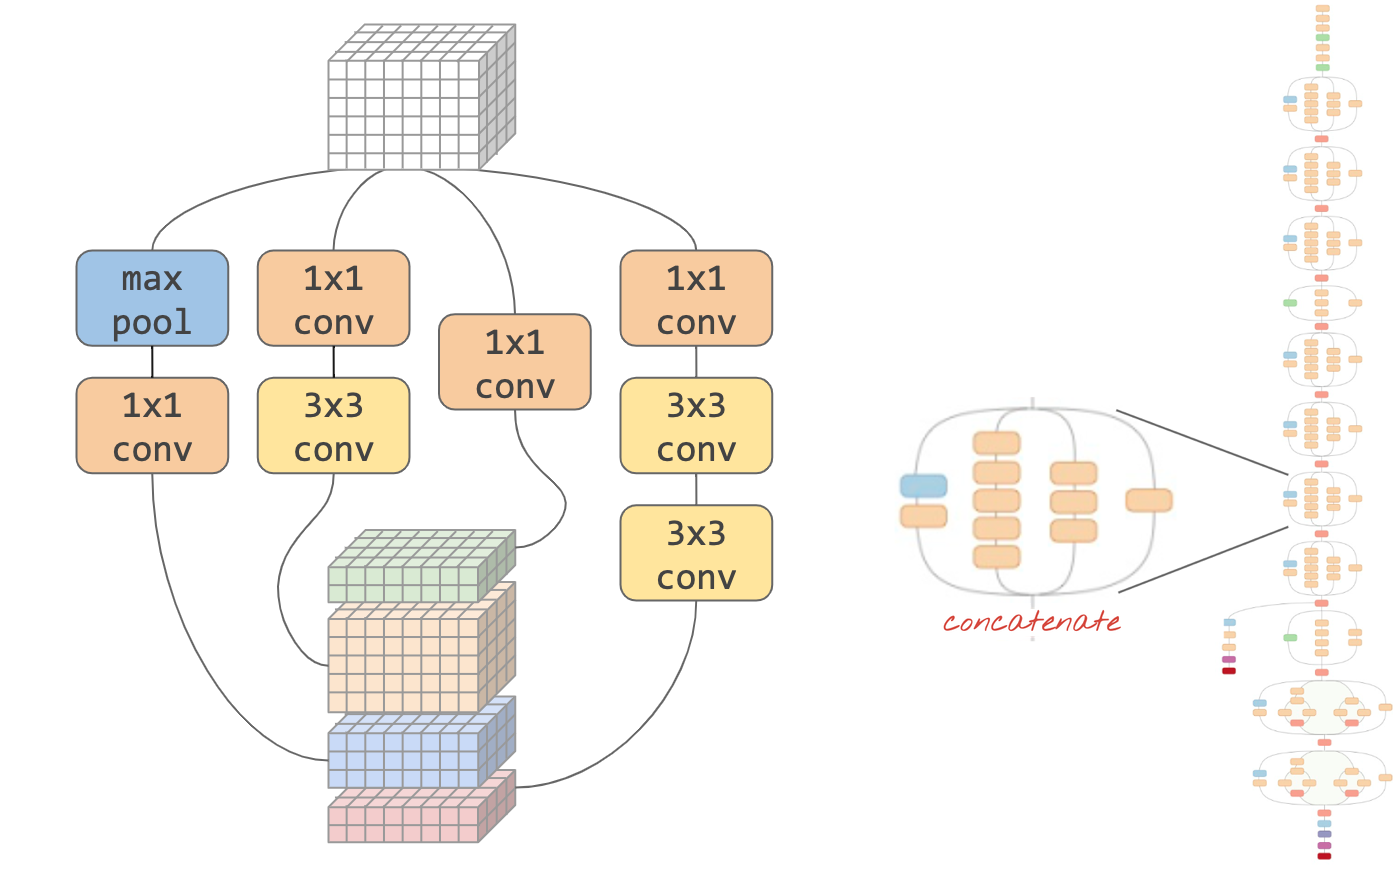
\includegraphics[width=0.82\textwidth]{Bilder/SqueezeNetModel.png}
    \caption{SqueezeNet}
    \label{fig:SqueezeNet}
\end{figure}


%!TEX root = ../documentation.tex
\chapter{Fazit}
\label{ch:conclusion}

\Blindtext

\begin{definition}[$\sigma$-Algebra]
    Sei $X$ eine Menge. Eine Teilmenge $\Sigma \in \mathcal{P}\left(X\right)$ heißt
    $\sigma$-Algebra wenn die folgenden drei Eigenschaften gelten: 
    \begin{enumerate}
        \item $X \in \Sigma$
        \item $A \in \Sigma \implies X \setminus A \in \Sigma$
        \item $A_1,A_2,\dots \in \Sigma \implies A_1 \cup A_2 \cup \dots \in \Sigma$
    \end{enumerate}
\end{definition}
Für eine Liste von Umgebungen siehe \texttt{preamble.tex}




% when adding a new chapter comment out this line
%\input{chapter/chapterFile.tex}

\appendix % hier beginnt der Anhang
%!TEX root = ../thesis.tex
\chapter{Ein Anhangskapitel}

\blindtext



\printbibliography

\end{document}
